\chapter{سخت‌افزار و الکترونیک}

همانطور که گفته شد، این پروژه شامل سه قسمت اصلی سخت‌افزار، مکانیک و نرم‌افزار است. در این فصل، به تشریح سخت‌افزار می‌پردازیم.

\section{فیبر مدارچاپی}
	فیبر مدار چاپی یا \pcb\footnote{\lr{Printed Circiut Board}} صفحه‌ای است معمولا از جنس فیبر \lr{FR-4} که با دو لایه‌ی نازک مس (معمولا به ضخامت 35 میکرون) در طرفین پوشیده است. طرحی که طراح به کارخانه‌ی چاپ \pcbf ارسال می‌کند روی این ورقه‌ها پیاده می‌شود. سپس لایه‌ی محافظ معمولا سبز رنگ به نام \lr{Solder mask} روی آن اضافه می‌شود که برای زیبایی بخشی به کار و محافظت از مس در مقابل خوردگی و اکسایش است.
	
	در این پروژه از یک \pcbf چهارلایه استفاده شده است. به دلیل فشردگی بالای طرح و قطعات، همچنین برای بهبود کیفیت سیگنال‌ها و کاهش اثر نویز، دو صفحه‌ی زمین در لایه‌های 2 و 3 تعبیه شده است. این صفحه‌ها با کوتاه کردن مسیر جریان برگشتی باعث بهبود کیفیت سیگنال و کاهش اثر نویز می‌شوند. همچنین تأثیر چشم‌گیری در سهولت مسیرکشی \pcbf دارند.

 \pcbf 
 های این پروژه -به رایگان- توسط شرکت \lr{PCBWay}\cite{PCBWay} چاپ شده است که از بزرگترین و مجهزترین کارخانه‌های چاپ \pcbf در کشور چین است.
 
 شکل \ref{fig:pcb_design}  تصویر \pcbf طراحی شده در نرم‌افزار \lr{Altium Designer} را نشان می‌دهد. تصاویر مربوط به \pcbf در شکل \ref{fig:pcb-images} قابل مشاهده است.
 
 \begin{figure}[h]
 	\centering
 	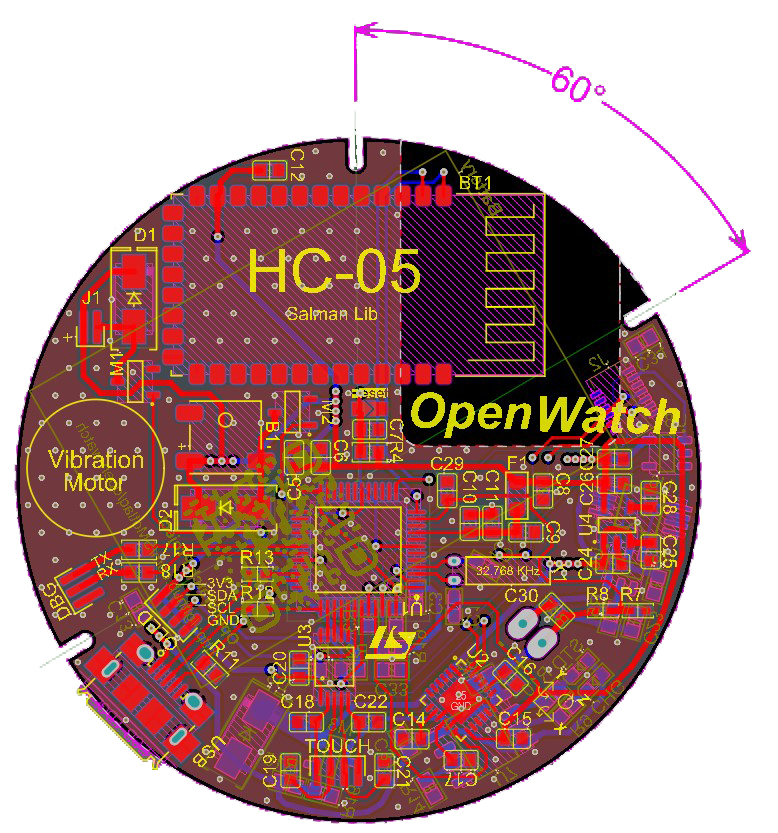
\includegraphics[width=0.5\textwidth]{pcb_main}
 	\caption{\pcbf طراحی شده در نرم‌افزار \lr{Altium Designer}}
 	\label{fig:pcb_design}
 \end{figure}
 
 \begin{figure}[h]
 	\centering
 	\begin{subfigure}{0.45\textwidth}
 		\centering
 		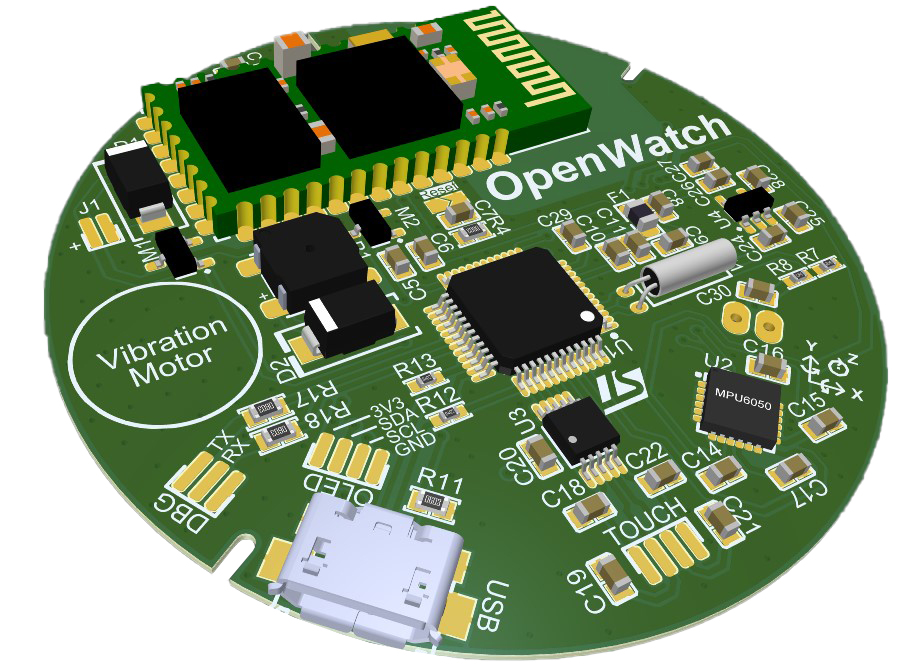
\includegraphics[width=0.9\linewidth]{pcb_main_3d}
 		\caption{نمای سه بعدی طرح - رو}
 		%\label{fig:stm32_image}
 	\end{subfigure}
 	\begin{subfigure}{0.45\textwidth}
 		\centering
 		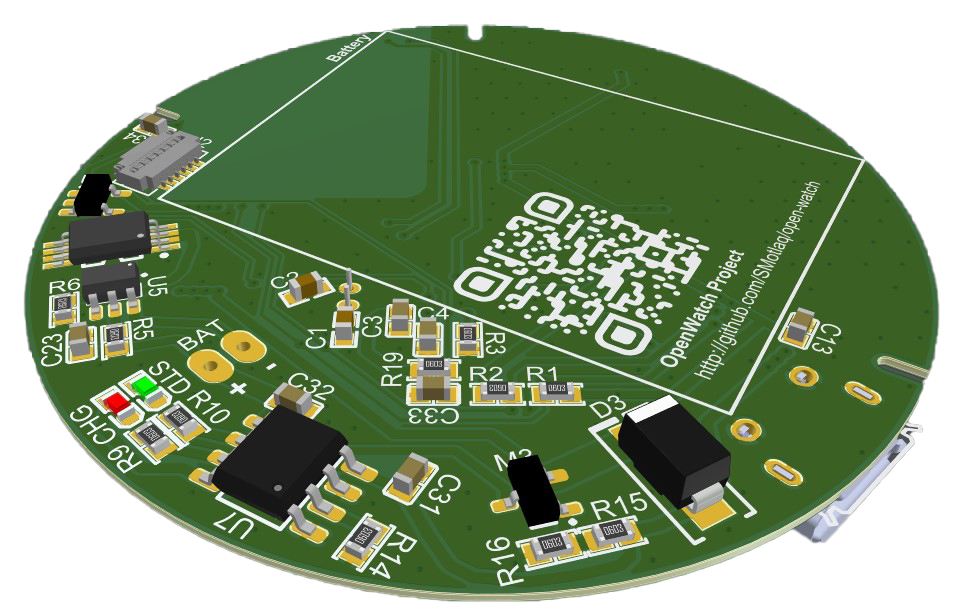
\includegraphics[width=\linewidth]{pcb_main_3d_back}
 		\caption{نمای سه بعدی طرح - پشت}
 		%\label{fig:stm32_real}
 	\end{subfigure}\\
	\begin{subfigure}{0.45\textwidth}
		\centering
		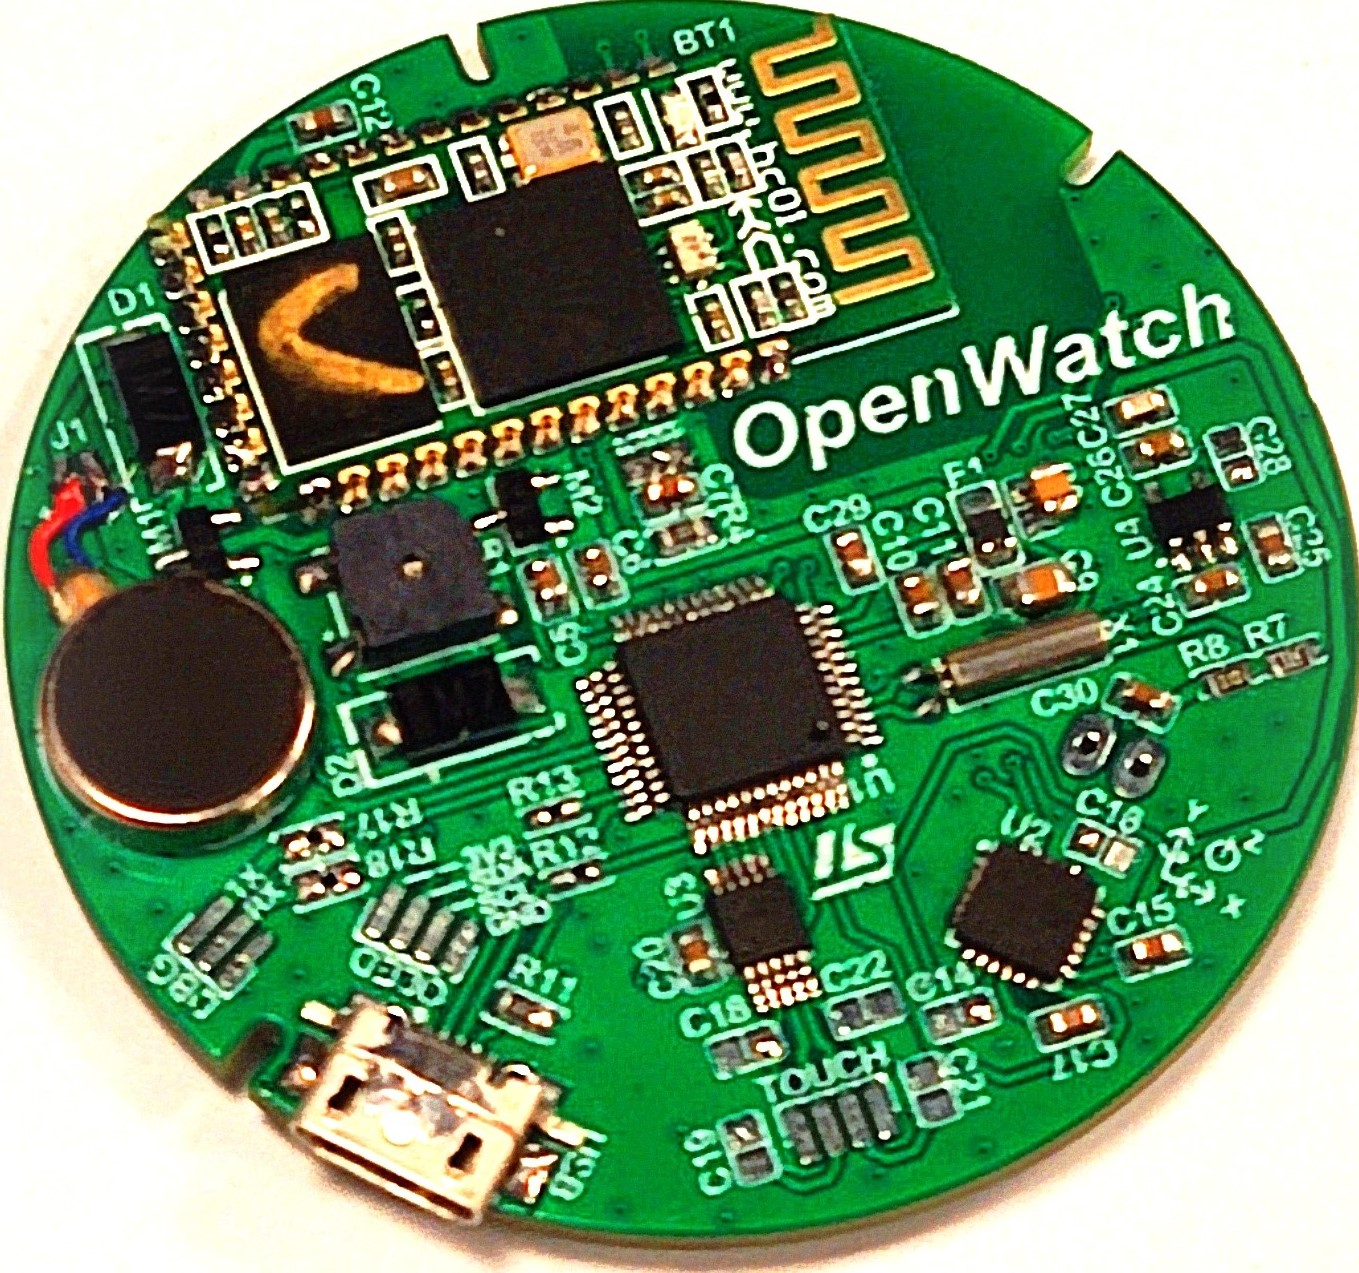
\includegraphics[width=0.9\linewidth]{pcb_real_mounted}
		\caption{\pcbf مونتاژ شده}
		%\label{fig:stm32_image}
	\end{subfigure}
	\begin{subfigure}{0.45\textwidth}
		\centering
		\includegraphics[width=0.9\linewidth]{pcb_real_raw}
		\caption{\pcbf خام}
		%\label{fig:stm32_image}
	\end{subfigure}
 	\caption{تصاویری از \pcbf پروژه}
 	\label{fig:pcb-images}
 \end{figure}
 
\section{هسته‌ی پردازشی} \label{sec:mcu}
برای انتخاب پردازنده‌ی مناسب باید موارد ذیل را مدنظر داشت:
\begin{enumerate}
	\item مقدار حافظه‌ی فلش\footnote{\lr{Flash}}:\\
	برنامه‌ای که برای پردازنده نوشته می‌شود در حافظه‌ی فلش ذخیره می‌شود. پس این حافظه مشخص می‌کند چه حجمی از برنامه در این پردازنده جا می‌شود.
	\item مقدار حافظه‌ی رم\footnote{\lr{RAM}}:\\
	این حافظه، یک حافظه‌ی موقت است که متغیرها، اشاره‌گرها\footnote{\lr{Pointers}}، نقطه‌ی بازگشت توابع و مقادیر ثبات‌ها\footnote{\lr{Registers}} به طور موقت در آن نوشته می‌شود. مقدار رم موردنیاز باید با توجه به حجم متغیرها و پیچیدگی عملیاتی و محاسباتی برنامه تعیین شود.
	\item تعداد پایه‌ها و مدارهای واسط\footnote{\lr{Peripherals}}:\\
	پردازنده‌های مختلف تنوع زیادی در نوع و تعداد مدارهای واسط ارائه می‌دهند. با توجه به تعداد سخت‌افزارهای جانبی، باید تعداد پایه و نوع مدارهای واسط موردنیاز تعیین شود.
	\item پکیج\footnote{\lr{Package}}:\\
	پکیج‌های مختلف نمایانگر شکل ظاهری پردازنده است. برخی پکیج‌ها ابعاد بزرگی دارند و برخی دیگر به قدری کوچک هستند که پایه‌های پردازنده در زیر تراشه تعبیه می‌شوند تا فضای کمتری اشغال کند. در انتخاب پکیج باید محدودیت فضای \pcbf را مدنظر قرار داد.
	\item موجودی بازار:\\
	یکی از مهمترین چالش‌های مهندسان الکترونیک در ایران، موجودی بازار است. خیلی از قطعاتی که طراح به آن‌ها نیاز دارد در بازار ایران پیدا نمی‌شود یا قیمت بالایی دارد. یا باید به وارد کردن قطعه و تاخیر چند ماهه تن داد یا باید طرح را عوض کرد تا با قطعات موجود در بازار قابل پیاده‌سازی باشد.
	\item قیمت:\\
	بدیهی است که یکی از قیود طراحی، قیمت تمام شده است. طراح باید در انتخاب پردازنده طوری عمل کند که با کمترین قیمت، بهترین تطابق را با قیود بالا ایجاد کند.
\end{enumerate}

در نهایت با بررسی موارد فوق، پردازنده‌ی انتخاب شده در این پروژه \lr{STM32F030C8} است. این پردازنده محصول شرکت \lr{ST} که هسته‌ی \lr{ARM Cortex-M0} 32 بیتی دارد. شکل \ref{fig:stm32_image} تصویر واقعی این پردازنده و شکل \ref{fig:stm32_real} تصویر آن را بر روی \pcbf ساعت نشان می‌دهد.

\begin{figure}[h]
	\centering
	\begin{subfigure}{0.35\textwidth}
		\centering
		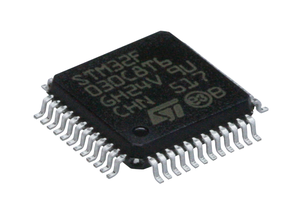
\includegraphics[width=\linewidth]{stm32f030}
		\caption{جداگانه}
		\label{fig:stm32_image}
	\end{subfigure}
	\begin{subfigure}{0.35\textwidth}
		\centering
		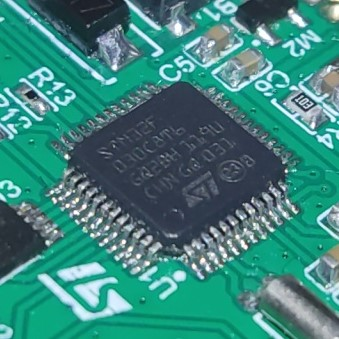
\includegraphics[width=\linewidth]{stm32f030_real}
		\caption{مونتاژ شده روی برد پروژه}
		\label{fig:stm32_real}
	\end{subfigure}
	\caption{تصاویری از پردازنده \lr{STM32F030}}
	\label{fig:stm32}
\end{figure}

شکل \ref{fig:sch-mcu} شماتیک مداری بخش پردازنده را نشان می‌دهد. یک کریستال 32768 هرتزی وظیفه‌ی تنظیم فرکانس بخش
 \lr{RTC}\footnote{\lr{Real Time Clock}}
  را بر عهده دارد. ساعت سیستم توسط این واحد ذخیره و تنظیم می‌شود. تغذیه‌ی بخش 
  \lr{ADC}\footnote{\lr{Analog to Digital Converter}}
  توسط چند خازن و یک فریت‌بید\footnote{\lr{Ferrite Bead}} فیلتر شده است. تغذیه‌ی خود پردازنده نیز توسط 4 خازن (مطابق با دستور کارخانه سازنده) فیلتر شده است.

\begin{figure}
	\centering
	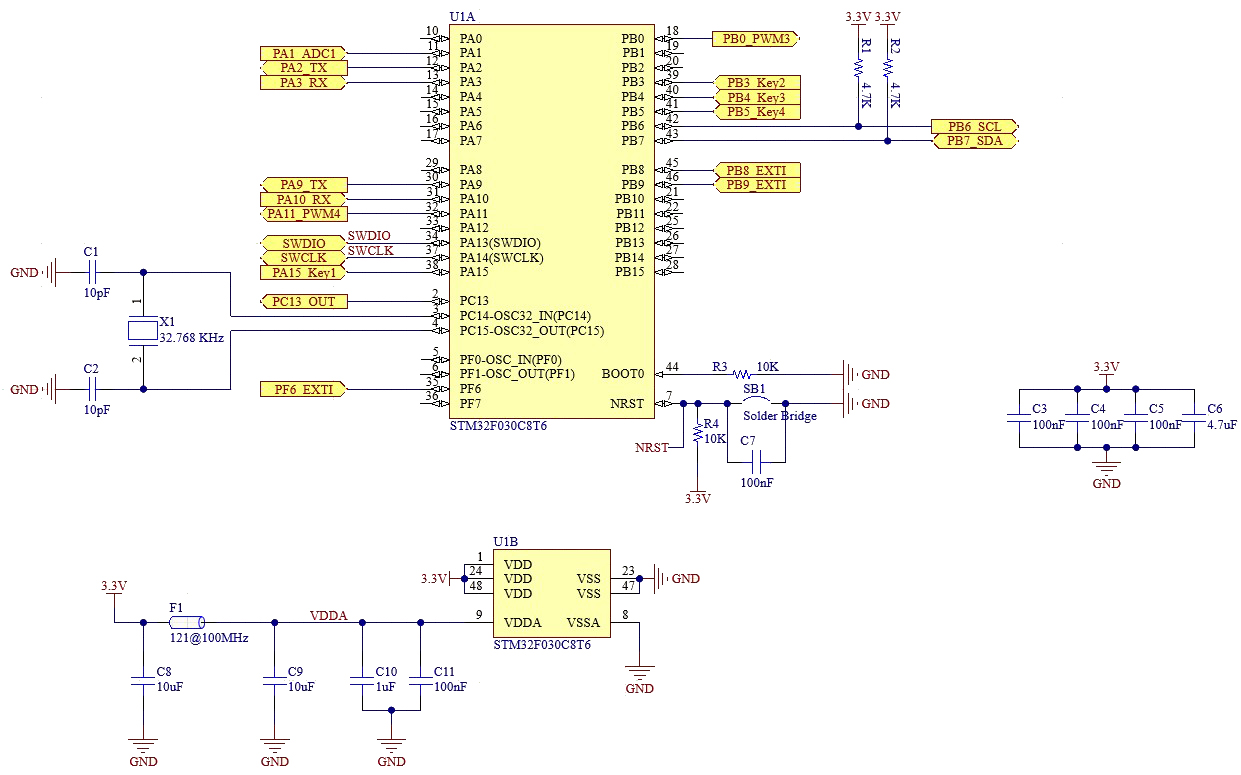
\includegraphics[width=\textwidth]{sch_mcu}
	\caption{شماتیک مربوط به بخش ریزپردازنده}
	\label{fig:sch-mcu}
\end{figure}


\section{درگاه بلوتوث}
ارتباط ساعت با تلفن‌همراه از طریق درگاه بلوتوث\footnote{\lr{Bluetooth}} است. قیود انتخاب بلوتوث هم تا حدی مشابه قیود انتخاب پردازنده (ابتدای بخش \ref{sec:mcu}) است. با در نظر گرفتن شرایط بازار، قیمت و عملکرد ماژول‌های مختلف، نهایتا ماژول \lr{HC-05} برای این پروژه انتخاب شد. شکل \ref{fig:hc05_image} تصویر این ماژول و شکل \ref{fig:hc05_real} تصویر آن را بر روی \pcbf ساعت نشان می‌دهد.

یکی از نکات مهمی که در طراحی \pcbf برای ماژول‌های مخابراتی وجود دارد این است که در نزدیکی آنتن این ماژول‌ها نباید هادی جریان الکتریکی وجود داشته باشد. در غیر این صورت خاصیت خازنی بین آنتن و این هادی باعث تغییر مشخصه‌های آنتن می‌شود و باعث اختلال در عملکرد آنتن می‌گردد. همانطور که در شکل \ref{fig:pcb_design} مشاهده می‌شود، مس‌های اطراف آنتن  حذف شده‌اند تا عملکرد بلوتوث دچار مشکل نشود.

\begin{figure}[h]
	\centering
	\begin{subfigure}{0.45\textwidth}
		\centering
		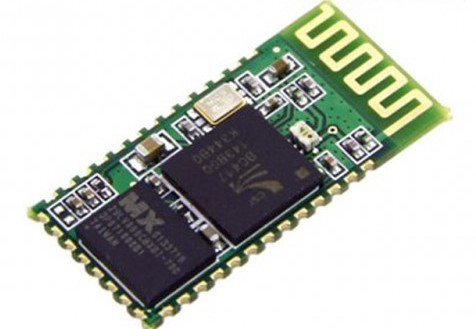
\includegraphics[width=\linewidth]{hc05_real}
		\caption{جداگانه}
		\label{fig:hc05_image}
	\end{subfigure}
	\begin{subfigure}{0.45\textwidth}
		\centering
		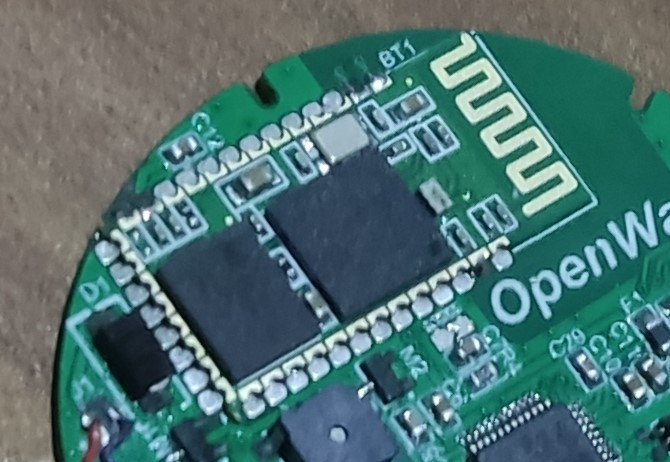
\includegraphics[width=\linewidth]{hc05_mounted}
		\caption{مونتاژ شده روی برد پروژه}
		\label{fig:hc05_real}
	\end{subfigure}
	\caption{تصاویری از ماژول بلوتوث \lr{HC-05}}
	\label{fig:hc05}
\end{figure}

شکل \ref{fig:sch-blue} شماتیک مداری بخش بلوتوث را نشان می‌دهد. پروتکل ارتباطی این ماژول با پردازنده پروتکل
 \lr{UART}\footnote{\lr{Universal Asynchronous Receiver-Transmitter}}
است که با دو پین \lr{RX} و \lr{TX} به پردازنده متصل می‌شود. پریفرال \lr{UART2} در پردازنده به ارتباط با بلوتوث اختصاص دارد. تغذیه‌ی ماژول نیز با یک خازن 100 نانوفارادی فیلتر شده است.

\begin{figure}[h]
	\centering
	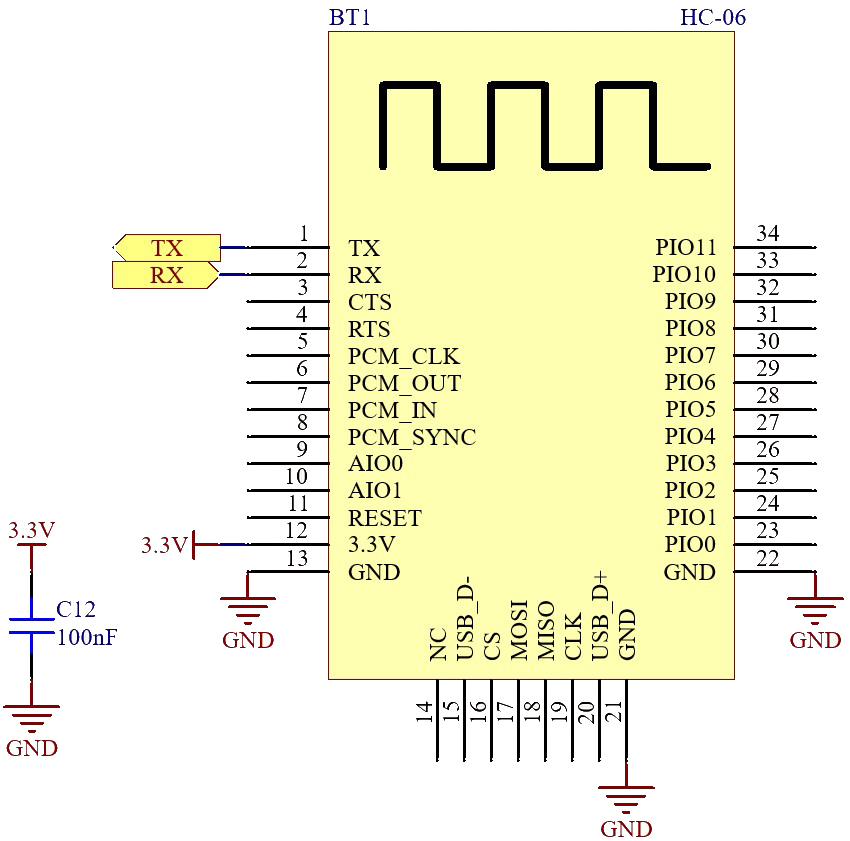
\includegraphics[width=0.6\textwidth]{sch_blue}
	\caption{شماتیک مربوط به بخش بلوتوث}
	\label{fig:sch-blue}
\end{figure}

\section{درگاه ارتباط سریال}
پریفرال \lr{UART1} در پردازنده با دو پین \lr{RX} و \lr{TX} از روی \pcbf خارج شده‌اند. کاربرد این دو پین اشکال‌یابی\footnote{\lr{Debug}} و ارتباط سرعت بالا بین ساعت و رایانه است. این بخش کاربردی در عملکرد کلی ساعت ندارد و صرفا روند توسعه را تسریع می‌کند. شکل \ref{fig:sch_debug} شماتیک مداری و شکل \ref{fig:debug_real} تصویر واقعی این دو پین را نشان می‌دهد.

\begin{figure}[h]
	\centering
	\begin{subfigure}{0.59\textwidth}
		\centering
		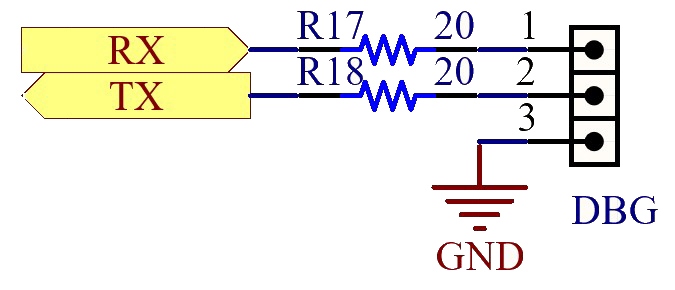
\includegraphics[width=\linewidth]{sch_debug}
		\caption{شماتیک}
		\label{fig:sch_debug}
	\end{subfigure}
	\begin{subfigure}{0.4\textwidth}
		\centering
		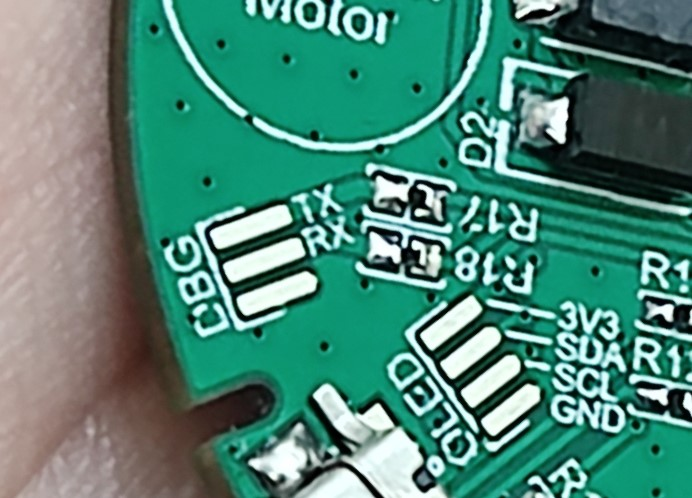
\includegraphics[width=\linewidth]{debug_real}
		\caption{پین‌های مربوطه}
		\label{fig:debug_real}
	\end{subfigure}
	\caption{تصاویر مربوط به درگاه ارتباط سریال}
\end{figure}

\section{حسگر پالس‌اکسی‌متر}
\newpage

\section{حسگر شتاب خطی و سرعت زاویه‌ای}
برای اندازه‌گیری مشخصه‌های حرکتی باید سراغ
\lr{IMU}\footnote{\lr{Inertial Measurement Unit}}ها
رفت. \lr{IMU}ها وسیله‌های الکترونیکی هستند که با استفاده‌ی ترکیبی از شتاب‌سنج‌ها، ژیروسکوپ‌ها و گاهی اوقات مغناطیس‌سنج‌ها، مشخصه‌های حرکتی را اندازه‌گیری و گزارش می‌کنند \cite{IMU}. در این پروژه از حسگر \lr{MPU6050} به این منظور استفاده شده است. این حسگر علی‌رغم قیمت نسبتا پایین، دقت و سرعت مناسبی دارد. مشخصات فنی این حسگر در ضمیمه ؟ موجود است. شکل \ref{fig:gyro_image} تصویر این حسگر و شکل \ref{fig:gyro_real} تصویر آن را بر روی \pcbf ساعت نشان می‌دهد.

\begin{figure}[h]
	\centering
	\begin{subfigure}{0.5\textwidth}
		\centering
		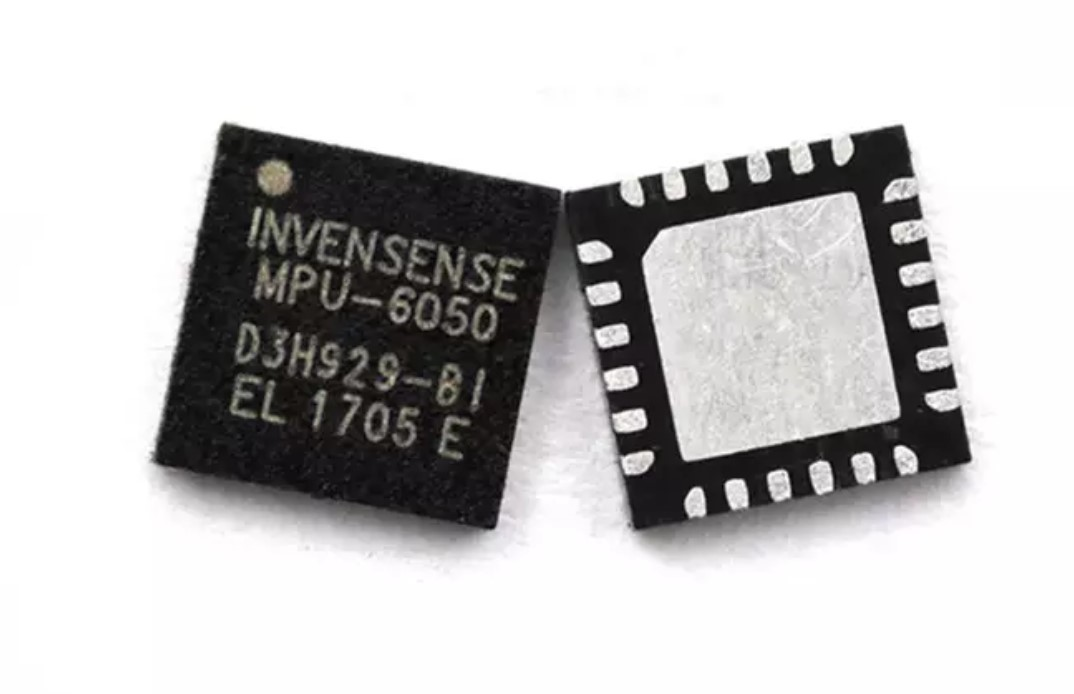
\includegraphics[width=\linewidth]{gyro_image}
		\caption{جداگانه}
		\label{fig:gyro_image}
	\end{subfigure}
	\begin{subfigure}{0.44\textwidth}
		\centering
		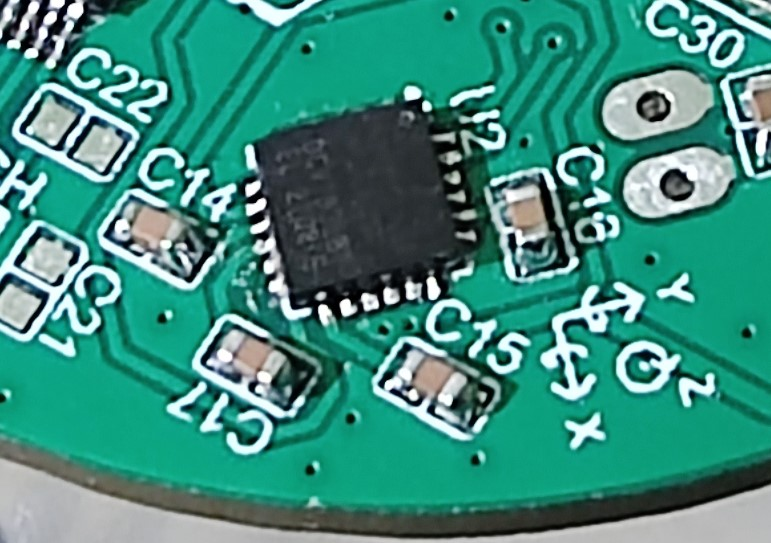
\includegraphics[width=\linewidth]{gyro_real}
		\caption{مونتاژ شده روی برد پروژه}
		\label{fig:gyro_real}
	\end{subfigure}
	\caption{تصاویر حسگر حرکتی}
	%	\label{fig:hc05}
\end{figure}

شکل \ref{fig:sch-gyro} شماتیک مداری حسگر \lr{MPU6050} را نشان می‌دهد. خازن‌ها طبق دستور کارخانه به حسگر متصل شده‌اند. درگاه ارتباطی این حسگر، باس\footnote{\lr{Bus}}
 \lr{I2C}\footnote{\lr{Inter-Integrated Circiut}}
  است. به همین دلیل \lr{I2C1} پردازنده به این حسگر متصل است.

\begin{figure}[h]
	\centering
	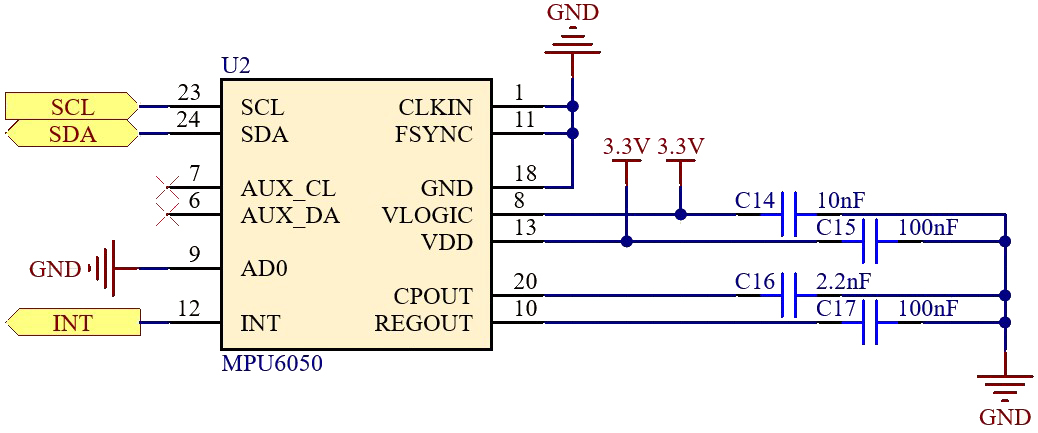
\includegraphics[width=0.8\textwidth]{sch_gyro}
	\caption{شماتیک مربوط به بخش حسگر حرکتی}
	\label{fig:sch-gyro}
\end{figure}

\section{صفحه نمایش}

\section{مدار شارژ و مدیریت توان}

\section{موتور ایجاد لرزش}
برای ایجاد لرزش\footnote{\lr{Vibration}} در ساعت، مشابه تلفن‌های همراه، از یک موتور مخصوص استفاده شده است. موتورهای ایجاد لرزش معمولا یک موتور \lr{DC} ساده هستند که یک بار نامتقارن به آن‌ها متصل است. از آنجا که مرکز جرم این بار خارج از شفت موتور است، چرخش آن باعث ایجاد گشتاوری دوار می‌شود که لرزش را ایجاد می‌کند. شکل \ref{fig:hc05_image} تصویر این موتور و شکل \ref{fig:hc05_real} تصویر آن را بر روی \pcbf ساعت نشان می‌دهد.

\begin{figure}[h]
	\centering
	\begin{subfigure}{0.35\textwidth}
		\centering
		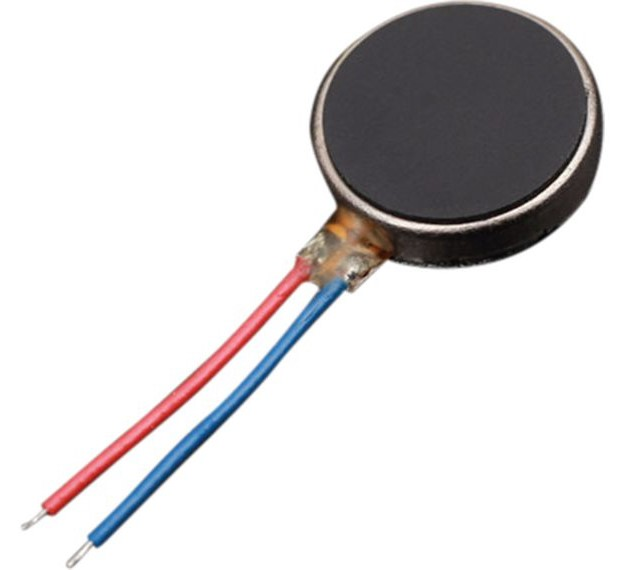
\includegraphics[width=0.75\linewidth]{vib_image}
		\caption{جداگانه}
		\label{fig:vib_image}
	\end{subfigure}
	\begin{subfigure}{0.44\textwidth}
		\centering
		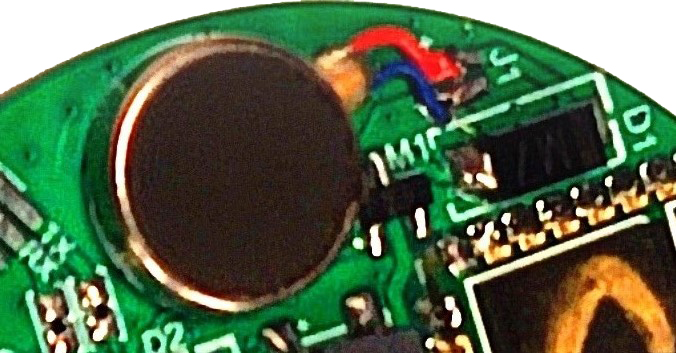
\includegraphics[width=\linewidth]{vib_real}
		\caption{مونتاژ شده روی برد پروژه}
		\label{fig:vib_real}
	\end{subfigure}
	\caption{تصاویر موتور ایجاد لرزش}
%	\label{fig:hc05}
\end{figure}

شکل \ref{fig:sch-vib} شماتیک مداری بخش ایجاد لرزش را نشان می‌دهد. این موتور برای کار به 90 میلی آمپر جریان الکتریکی احتیاج دادر. طبیعتا پردازنده نمی‌تواند این جریان را تأمین کند. لذا از یک سوییچ ماسفت
\footnote{\lr{Metal–Oxide–Semiconductor Field-Effect Transistor}}
 برای قطع و وصل موتور استفاده شده است. دیودی که با موتور موازی شده از ورود جریان برگشتی موتور به ماسفت هنگام خاموش شدن موتور جلوگیری می‌کند. برای کنترل سرعت موتور می‌توان از اعمال موج \lr{PWM}\footnote{\lr{Pulse Width Modulation}} به موتور بهره برد. لذا پایه‌ی فرمان این مدار به خروجی \lr{PWM} تایمر 1 در پردازنده متصل شده است.

\begin{figure}[h]
	\centering
	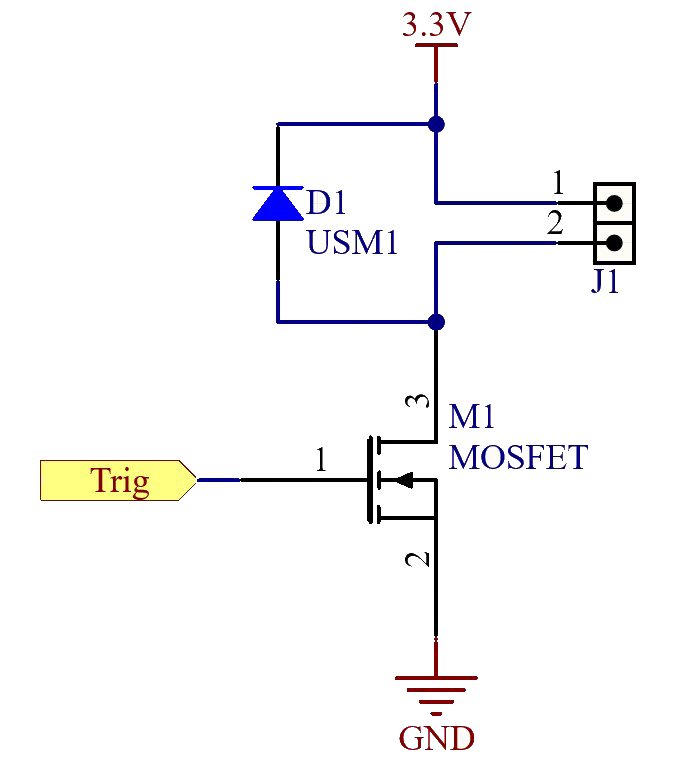
\includegraphics[width=0.52\textwidth]{sch_vib}
	\caption{شماتیک مربوط به بخش ایجاد لرزش}
	\label{fig:sch-vib}
\end{figure}

\section{بازر}

\section{کلیدهای لمسی}